\usepackage{xcolor}
\usepackage{afterpage}
\usepackage{pifont,mdframed}
\usepackage[bottom]{footmisc}


\createsection{\Grader}{Grader di prova}
\createsection{\Specs}{Chiarimenti}

\renewcommand{\inputfile}{\texttt{stdin}}
\renewcommand{\outputfile}{\texttt{stdout}}
\makeatletter
\renewcommand{\this@inputfilename}{\texttt{stdin}}
\renewcommand{\this@outputfilename}{\texttt{stdout}}
\makeatother

\newenvironment{warning}
  {\par\begin{mdframed}[linewidth=2pt,linecolor=gray]%
    \begin{list}{}{\leftmargin=1cm
                   \labelwidth=\leftmargin}\item[\Large\ding{43}]}
  {\end{list}\end{mdframed}\par}

\newenvironment{todoenv}
{\par\begin{mdframed}[linewidth=2pt,linecolor=red]%
		\begin{list}{}{\leftmargin=1cm
				\labelwidth=\leftmargin}\item[\Large\ding{169}]}
		{\end{list}\end{mdframed}\par}

\newcommand{\todo}[1]{\begin{todoenv}
		TODO: #1
\end{todoenv}}

% % % % % % % % % % % % % % % % % % % % % % % % % % % % % % % % % % % % % % % % % % %
% % % % % % % % % % % % % % % % % % % % % % % % % % % % % % % % % % % % % % % % % % %


Come da tradizione OII, il giorno di gara precede la lunga notte di
festeggiamenti. Quest'anno verrà organizzato un party sfrenato
in perfetto stile trentino, durante il quale i ragazzi e le ragazze si daranno alla
pazza gioia. Ovviamente, per ``pazza gioia'' intendiamo cimentarsi in
un'attività intellettualmente stimolante ed allo stesso tempo non troppo
faticosa!

Quest'anno, la scelta dell'attività è ricaduta su un passatempo piuttosto
sofisticato: costruire una lunghissima catena di domino.

\begin{wrapfigure}[10]{r}{0.4\textwidth}
  \vspace{-30pt}
  \begin{center}
    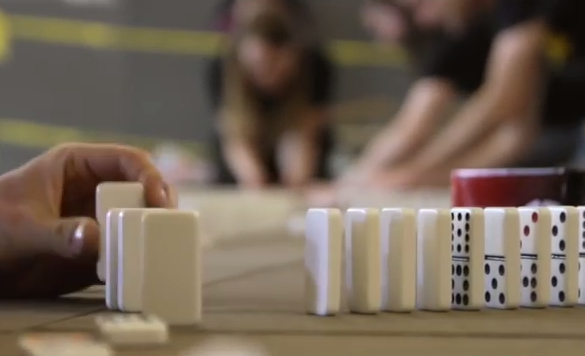
\includegraphics[width=0.9\linewidth]{domino.png}
    \caption{Atleti all'opera}
  \end{center}
\end{wrapfigure}

La festa si protrae per tutta la notte e viene bruscamente interrotta quando Monica
arriva a richiamare gli atleti per portarli al liceo Galilei, dove si terrà la
cerimonia di premiazione.

Finora gli atleti sono riusciti a posizionare in tutto $N$ tessere, ognuna ad
esattamente un centimentro di distanza dalla precedente. Non avendo a
disposizione abbastanza tessere tradizionali, hanno usato un po' di tutto:
ciascuna ``tessera'' potrebbe perciò essere alta pochi centimetri ma anche
svariati metri!

Per non vanificare gli sforzi fatti, gli atleti vogliono ora concludere la festa
in grande stile spingendo la prima tessera così da far cadere l'intera catena.
La caduta di una tessera alta $h$ fa cadere le successive $h-1$ tessere: quindi
le tessere di altezza $1$ non fanno cadere alcuna tessera.

Nella stanchezza della nottata, gli atleti temono di aver commesso qualche
errore nel posizionare le tessere. Non c'è però tempo di rifare tutto: aiutali a
capire se è possibile scambiare due tessere qualsiasi (ma solo due) in modo che
l'intera catena venga abbattuta!

\begin{mdframed}[backgroundcolor=black!10,rightline=false,leftline=false]

\Specs

\small

Le posizioni in cui si trovano le tessere sono numerate da $0$ a $N-1$.
Le posizione $0$ è quella più a sinistra e
le tessere cadono da sinistra verso destra.

Dopo aver effettuato l'eventuale scambio,
la tessera in posizione $0$ viene fatta cadere per prima.
Se la tessera in posizione $i$ cade,
ed è alta $h$,
allora cadranno anche tutte le tessere che si trovano nelle
posizioni fino a $i+h-1$, inclusa.

Quindi, la tessera in posizione $0$ cade sempre,
e una tessera in posizione $i \geq 1$
cade se e solo se esiste una tessera
in posizione $i' < i$,
che cade, alta almeno $i-i'+1$.

Nota che tutte le tessere cadono
se e solo se cade la tessera in posizione $N-1$.

\end{mdframed}

\pagebreak

% % % % % % % % % % % % % % % % % % % % % % % % % % % % % % % % % % % % % % % % % % %
% % % % % % % % % % % % % % % % % % % % % % % % % % % % % % % % % % % % % % % % % % %

\Implementation

Dovrai sottoporre un unico file, con estensione \texttt{.cpp} o \texttt{.c}.

\begin{warning}
Tra gli allegati a questo task troverai un template \texttt{catena.cpp} e \texttt{catena.c}
con un esempio di implementazione.
\end{warning}

Dovrai implementare la seguente funzione.

\begin{center}\begin{tabularx}{\textwidth}{|c|X|}
\hline
C/C++  & \verb|stato_t correggi(int N, int altezze[], coppia_t* scambio);|\\
\hline
\end{tabularx}\end{center}

\begin{itemize}[nolistsep]
  \item L'intero $N$ rappresenta il numero di tessere.
  \item
    L'array \texttt{altezze}, indicizzato da $0$ a $N-1$, contiene l'altezza di ciascuna tessera.
    La tessera inizialmente in posizione $i$, con $0 \leq i \leq N-1$, è alta $\texttt{altezze}[i]$.
  \item
    Il tipo di dato \texttt{stato\_t} è una \texttt{enum} che può assumere i valori
    \texttt{OK}, \texttt{RISOLTO} o \texttt{IMPOSSIBILE}.
    La funzione deve restituire:
    \begin{itemize}
      \item \texttt{OK}, se non è necessario alcuno scambio affinché cadano tutte le tessere; altrimenti,
      \item \texttt{RISOLTO},
        se è possibile scambiare due tessere,
        in modo che dopo lo scambio tutte le tessere cadano; altrimenti,
      \item \texttt{IMPOSSIBILE},
        quando un singolo scambio non è sufficiente.
    \end{itemize}
  \item
    Il tipo di dato \texttt{coppia\_t} è una \texttt{struct} che contiene i campi
    \texttt{domino1} e \texttt{domino2}.
    Qualora la funzione restituisca \texttt{RISOLTO},
    i campi \texttt{domino1} e \texttt{domino2}
    del parametro di output \texttt{scambio}
    devono essere riempiti con le posizioni
    delle due tessere da scambiare.
\end{itemize}

La funzione \texttt{correggi} sarà chiamata una sola volta.
Sarà registrato il valore di ritorno della funzione e,
se questo valore è \texttt{RISOLTO},
anche le posizioni memorizzate nella struttura \texttt{scambio}.

% % % % % % % % % % % % % % % % % % % % % % % % % % % % % % % % % % % % % % % % % % %
% % % % % % % % % % % % % % % % % % % % % % % % % % % % % % % % % % % % % % % % % % %


\Grader
Nella directory relativa a questo problema è presente una versione semplificata del grader usato durante la correzione, che potete usare per testare le vostre soluzioni in locale. Il grader di esempio legge i dati da \inputfile{}, chiama le funzioni che dovete implementare e scrive su \outputfile{}, secondo il seguente formato.

Il file di input è composto da $2$ righe, contenenti:
\begin{itemize}[nolistsep,itemsep=2mm]
\item Riga $1$: il numero intero $N$;
\item Riga $2$: i numeri interi \texttt{altezze[$i$]}, per $i = 0\ldots N-1$, separati da spazi.
\end{itemize}

Il file di output è composto da una sola riga che contiene una tra le seguenti possibilità:
\begin{itemize}[nolistsep,itemsep=2mm]
\item la stringa \texttt{OK}, se la catena di domino viene completamente abbattuta senza effettuare alcuno scambio;
\item la stringa \texttt{IMPOSSIBILE}, se non è possibile aggiustare la catena con un solo scambio;
\item due numeri interi $i$ e $j$, separati da spazio,
  se è possibile aggiustare la catena scambiando le tessere nelle posizioni $i$ e $j$.
\end{itemize}

% % % % % % % % % % % % % % % % % % % % % % % % % % % % % % % % % % % % % % % % % % %
% % % % % % % % % % % % % % % % % % % % % % % % % % % % % % % % % % % % % % % % % % %

\pagebreak
\Constraints

\begin{itemize}[nolistsep, itemsep=2mm]
	\item $1 \le N \le 5\,000\,000$.
	\item $1 \le \texttt{altezze}[i] \le 1000$ per ogni $i=0, \ldots, N-1$.
\end{itemize}

% % % % % % % % % % % % % % % % % % % % % % % % % % % % % % % % % % % % % % % % % % %
% % % % % % % % % % % % % % % % % % % % % % % % % % % % % % % % % % % % % % % % % % %


\Scoring

Il tuo programma verrà testato su diversi test case raggruppati in subtask.
Per ottenere il punteggio relativo ad un subtask, è necessario risolvere correttamente tutti i test che lo compongono.

\begin{itemize}[nolistsep,itemsep=2mm]
  \item \textbf{\makebox[2cm][l]{Subtask 1} [\phantom{0}0 punti]}: Casi d'esempio.
  \item \textbf{\makebox[2cm][l]{Subtask 2} [\phantom{0}4 punti]}: Le altezze sono tutte uguali.
  \item \textbf{\makebox[2cm][l]{Subtask 3} [\phantom{0}7 punti]}: $N \le 5000$ e la risposta è \texttt{OK} o \texttt{IMPOSSIBILE}.
  \item \textbf{\makebox[2cm][l]{Subtask 4} [\phantom{0}9 punti]}: La risposta è \texttt{OK} o \texttt{IMPOSSIBILE}.
  \item \textbf{\makebox[2cm][l]{Subtask 5} [13 punti]}: $N \leq 50$.
  \item \textbf{\makebox[2cm][l]{Subtask 6} [19 punti]}: $N \leq 1000$.
  \item \textbf{\makebox[2cm][l]{Subtask 7} [28 punti]}: $N \leq 3000$.
  \item \textbf{\makebox[2cm][l]{Subtask 8} [11 punti]}: $N \leq 100\,000$.
  \item \textbf{\makebox[2cm][l]{Subtask 9} [\phantom{0}9 punti]}: Nessuna limitazione specifica.
\end{itemize}

% % % % % % % % % % % % % % % % % % % % % % % % % % % % % % % % % % % % % % % % % % %
% % % % % % % % % % % % % % % % % % % % % % % % % % % % % % % % % % % % % % % % % % %


\Examples

\begin{example}
\exmpfile{caduta.input0.txt}{caduta.output0.txt}%
\exmpfile{caduta.input1.txt}{caduta.output1.txt}%
\exmpfile{caduta.input2.txt}{caduta.output2.txt}%
\end{example}

% % % % % % % % % % % % % % % % % % % % % % % % % % % % % % % % % % % % % % % % % % %
% % % % % % % % % % % % % % % % % % % % % % % % % % % % % % % % % % % % % % % % % % %

\pagebreak
\Explanation

Nel \textbf{primo caso di esempio} è sufficiente scambiare le tessere nelle posizioni $2$ e $3$:

\begin{center}
	\includegraphics[scale = 1.5]{asy_caduta/fig1.pdf}
\end{center}

Nel \textbf{secondo caso di esempio} la tessera in posizione $2$ è alta abbastanza: la catena va bene così com'è.

\begin{center}
	\includegraphics[scale = 1.5]{asy_caduta/fig2.pdf}
\end{center}

Nel \textbf{terzo caso di esempio} le tessere sono troppo basse: la catena non può cadere.

\begin{center}
	\includegraphics[scale = 1.5]{asy_caduta/fig3.pdf}
\end{center}
